\documentclass[report.tex]{subfiles}

\begin{document}

\chapter{On MCMC Output Analysis}
\label{mcmc-output-analysis}

In this chapter we present the basic theory behind the tools implemented in our
output analysis framework that can be used to objectively compare different
MCMC algorithms. We refer to
\citet[Chapter 1]{brooks2011handbook} and \citet[Chapter 5]{liu2008monte}, where
more thorough treatment of the following material can be found.

Suppose we have generated $n$ random samples $x^{(1)}, x^{(2)}, \dots, x^{(n)}$ using
some MCMC sampler with invariant distribution $\pi$ and further assume that
$x^{(1)} \sim \pi$ (usually obtained by throwing away some initial part of the
simulation, waiting for the Markov chain to converge to $\pi$).
Then, for an arbirary function $f$, we can estimate \exWithDistribution{\pi}{f(X)} by:
$$
\hat{\mu}_{n} \coloneqq \frac{1}{n} \sum_{i=1}^{n} f(x^{(i)}).
$$
Had our samples been independent, we would have
$\variance{\hat{\mu}_{n}} = \frac{1}{n} \varianceWithDistribution{\pi}{f(X)}$.
Unfortunatelly, samples drawn from a Markov chain are generally not independent.
Under certain regularity conditions, the Markov chain CLT tells us that as $n \to \infty$:
\begin{equation}
\label{asymptotic-variance}
\variance{\hat{\mu}_{n}} = \frac{\sigma_{f}^{2}}{n} = \frac{1}{n}(
  \varianceWithDistribution{\pi}{f(X)}
  + 2 \sum_{k=1}^{\infty} \covariance{f(X_{1})}{f(X_{1+k})})
\end{equation}
where $X_{1}, X_{2}, \dots$ is the Markov chain (with $X_{1} \sim \pi$) from
which we generate the samples.
The term denoted by $\sigma_{f}^{2}$ in Equation~\ref{asymptotic-variance}
is called the \textit{asymptotic variance}.
Essentially, if we want to compare two MCMC algorithms which generate samples
from the same distribution at the same speed, the one with lower asymptotic variance
is better since it provides a more reliable expectation estimator.

\section{Autocorrelation Function}

Let $\rho_{k} \coloneqq \corr{X_{1}}{ X_{1+k}}$ and call it \textit{lag-k autocorrelation}.
We can then rewrite Equation~\ref{asymptotic-variance}
as follows:
\begin{equation}
\label{asymptotic-variance-autocorrelation-time}
\variance{\hat{\mu}_{n}} = \frac{\varianceWithDistribution{\pi}{f(X)}}{n}(
1 + 2 \sum_{k=1}^{\infty} \rho_{k}).
\end{equation}
Hence, to compare two MCMC algorithms generating samples from the same distribution
we can simply plot their autocorrelation functions, which act as a proxy for estimating
the asymptotic variance.
See Figure~\ref{image-autocorrelation-function-example} for an example.

However, such an analysis does not take the speed of the samplers into account.
To see why it is problematic, consider the following scenario: samples generated using
one MCMC algorithm may possess bigger correlation than samples produced by another algorithm.
However, assume that the first algorithm generates the samples much faster. Then
it may still be preferable to use the first algorithm, which could produce better
expecatation estimates within a fixed time budget.
This issue is solved by comparing how many effective samples each
algorithm produces per time unit. See the next section for details.

Finally, we want to briefly discuss how to calculate the autocorrelation
function. Essentially, what we want to do is estimate $\rho_{k}$ for any given
value of $k$ (up to some upper bound for which we want to generate our plots).
Recall that:
$$
\rho_{k} = \frac{\covariance{f(X_{1})}{f(X_{1 + k})}}{\varianceWithDistribution{\pi}{f(X)}}
$$
so after generating $n$ samples from our MCMC algorithm, we can estimate $\rho_{k}$
by computing:
\begin{equation}
\label{correlation-estimator}
\sum_{i=1}^{n-k} \frac{(x^{(i)} - \hat{\mu}_{n})(x^{(i+k)} - \hat{\mu}_{n})}{\hat{\sigma}_{n}^{2}}
\end{equation}
where we estimate $\hat{\sigma}_{n}^{2}$ from our MCMC output simply in the same way as we estimate
any other expectation.

Recall that in our framework we implement an output processor which calculates autocorrelation
statistics online.
We face one difficulty, however, because we cannot reliably estimate $\hat{\mu}_{n}$
and $\hat{\sigma}_{n}^{2}$ at the beginning of the simulation.
Even though this is not ideal, to solve this problem we simply start estimating
the correlations after our output processor has obtained a pre-specified number
of samples (e.g. a trajectory of length 1000 was already generated).
We can then use these samples to get initial estimates of $\hat{\mu}_{n}$ and
$\hat{\sigma}_{n}^{2}$ and start using the estimator from Equation~\ref{correlation-estimator}.
As the simulation progresses, we keep updating the values of $\hat{\mu}_{n}$ and $\hat{\sigma}_{n}^{2}$
so that we get better and better estimates with the later samples.
Such procedure results in an online computation of autocorrelation function at the
cost of some extra noise.

\begin{SCfigure}
  \centering
  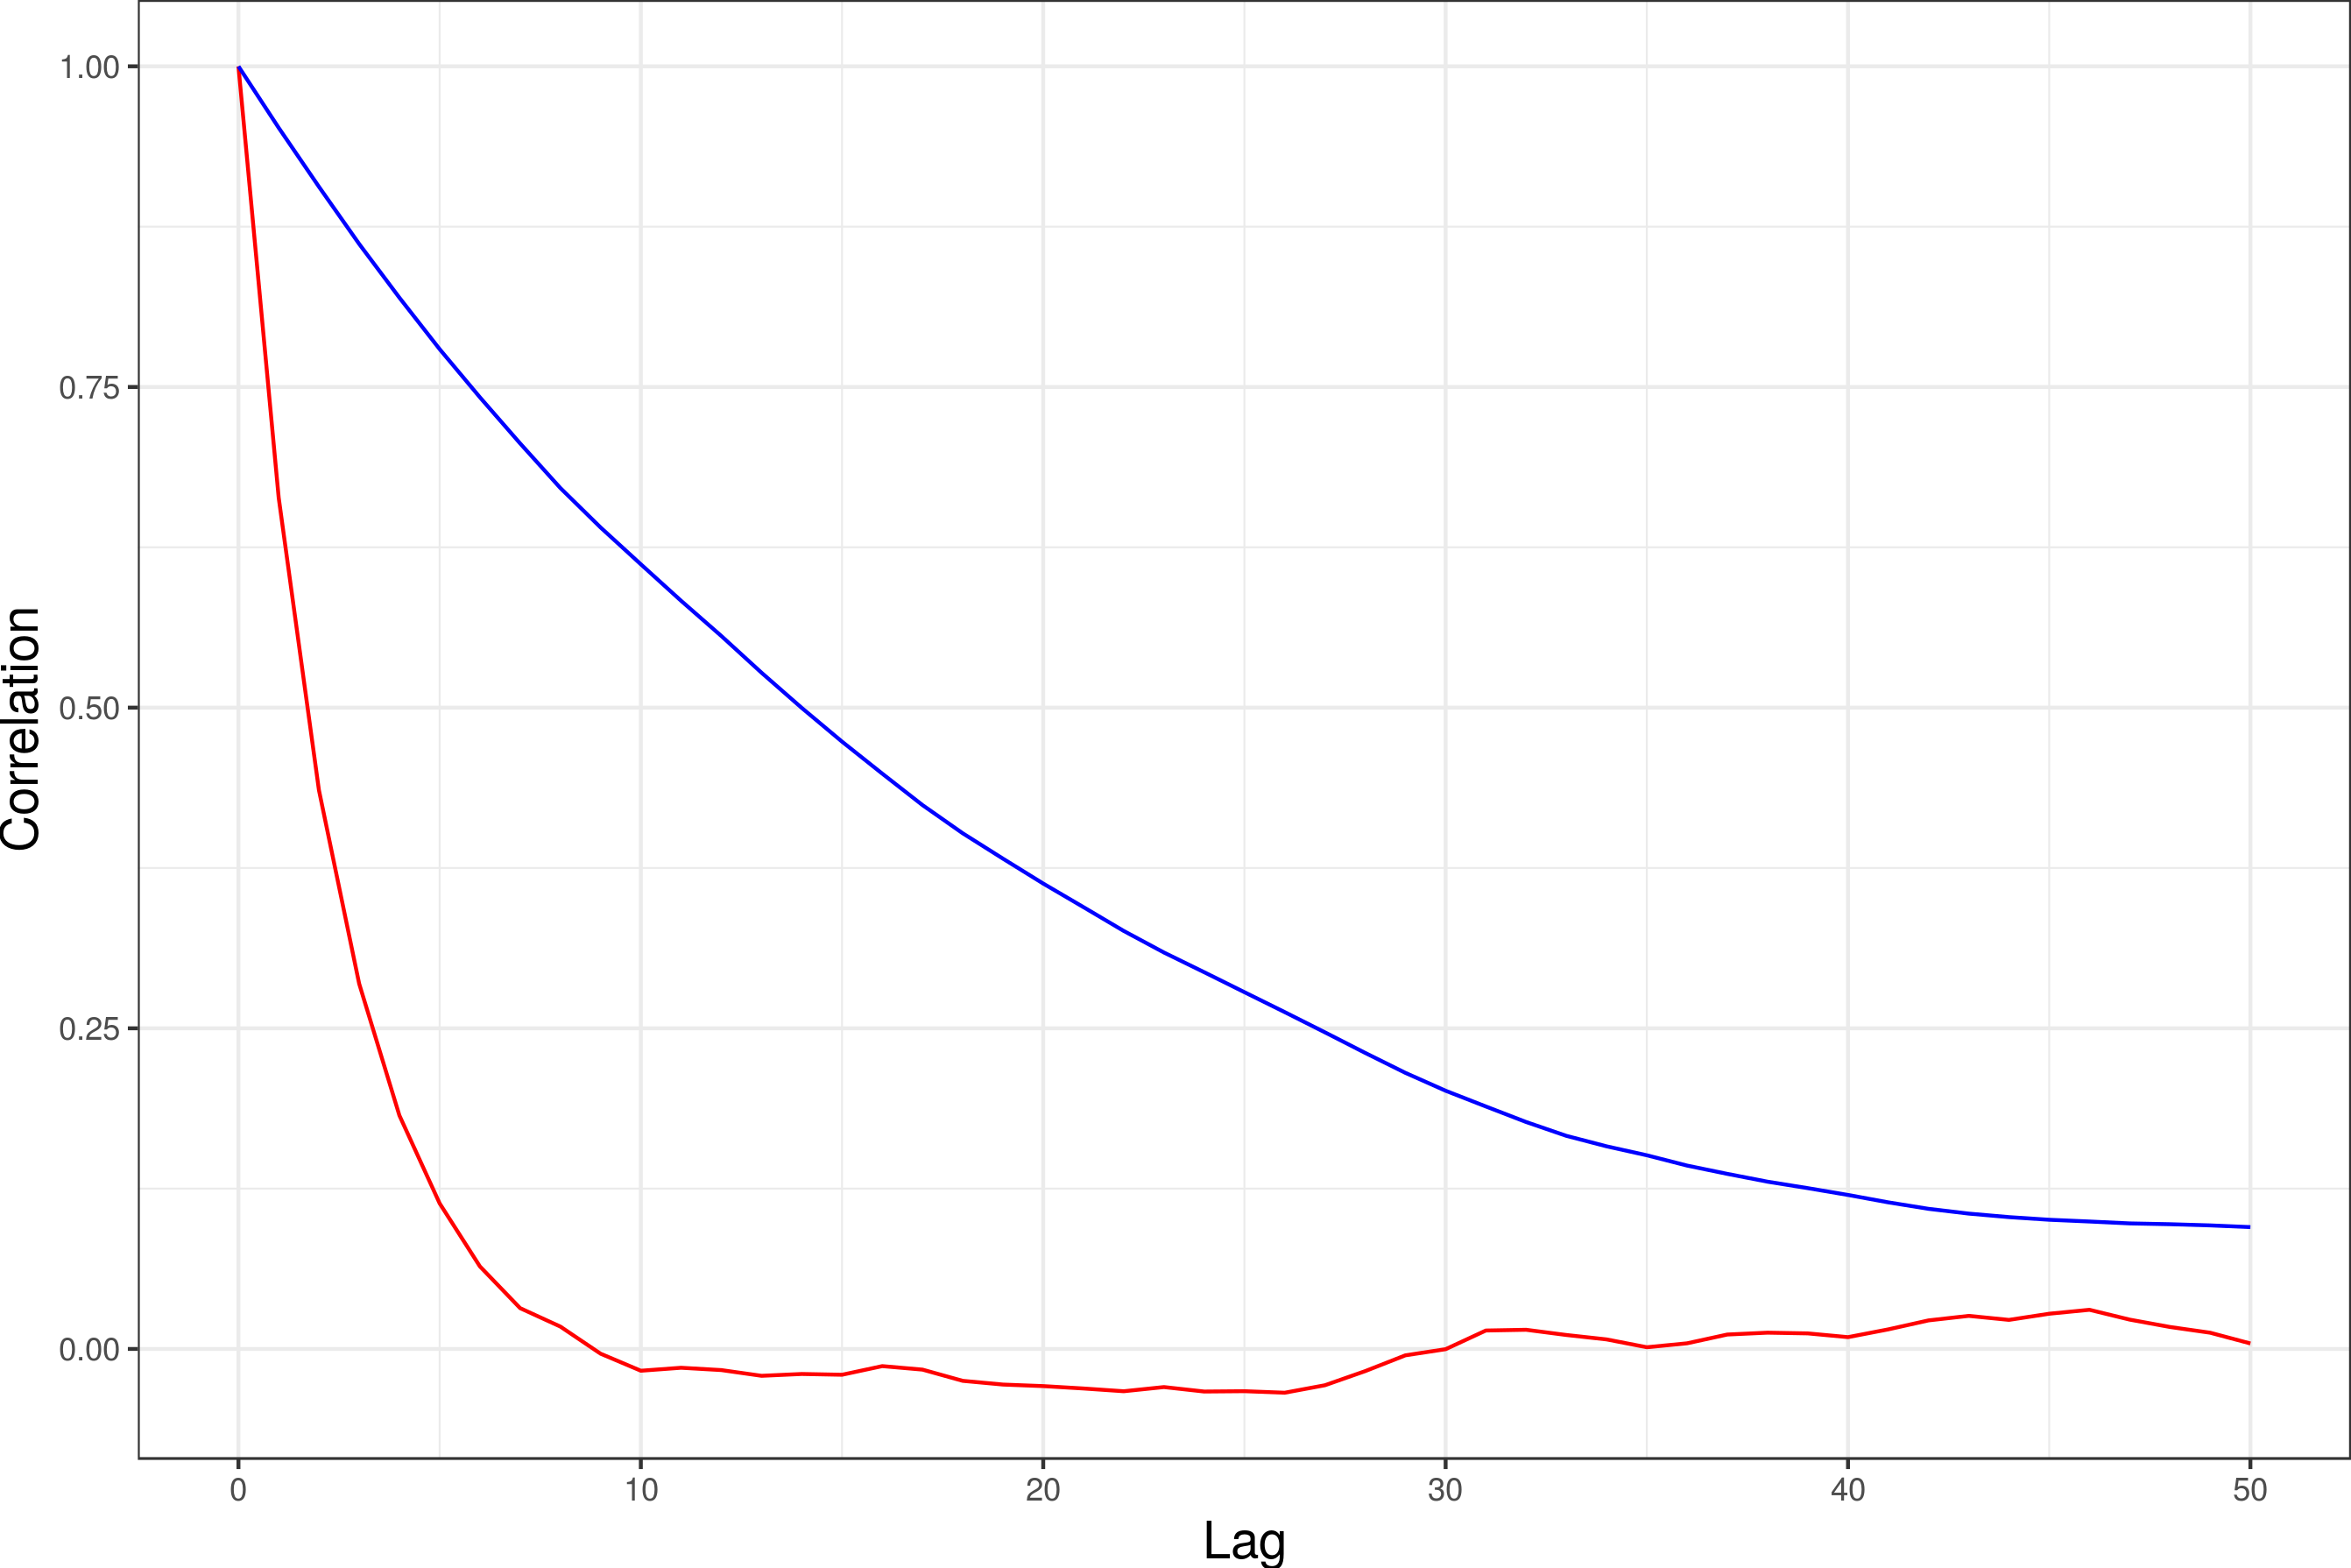
\includegraphics[width=0.5\textwidth]{img/appendix-autocorrelations-example}
  \caption{An example of autocorrelation plots. We simulate two Markov chains to generate
    samples from $N(0, 1)$ distribution according to the Metropolis scheme described in
    Equation~\ref{metropolis-acceptance-rate}, with proposal densities $q(\cdot \vert x) = N(x, \sigma^{2}).$
    The red curve is the autocorrelation function of the samples produces by such a MCMC
    algorithm using $\sigma^{2} = 1$.
    The blue curve was generated using $\sigma^{2} = 0.1$.
    It is easy to see from the grap, that
    setting $\sigma^{2}$ to $0.1$ results in too slow exploration of the state space.}
  \label{image-autocorrelation-function-example}
\end{SCfigure}


\section{Effective Sample Size}
As we have briefly mentioned already, we would like to have some way to compare MCMC algorithms
which also takes the running time into account. Define the \textit{integrated autocorrelation time}
(IACT) as:
$$
\tau_{\text{int}} \coloneqq 1 + 2 \sum_{k = 1}^{\infty} \rho_{k}.
$$
Now note that by Equation~\ref{asymptotic-variance-autocorrelation-time},
having $n \tau_{\text{int}}$ samples from our MCMC algorithm has the same effect
(in terms of variance of our expectation estimator) as having $n$ independent samples
from our target distribution $\pi$.
Hence, we define the \textit{effective sample size} of $n$ samples obtained from our simulated
Markov chain by the following equation:
$$
n_{\text{eff}} \coloneqq \frac{n}{\tau_{\text{int}}}.
$$
To compare the performance of different MCMC algorithms we can then run them
for the same amount of time and compare the number of effective samples produced
by each algorithm.

A question remains, however, of how to compute the $\tau_{\text{int}}$ which contains
an infinite sum in its expression.
Note that
$$
\tau_{\text{int}} = \frac{\sigma_{f}^{2}}{\varianceWithDistribution{\pi}{f(X)}}
$$
where $\sigma_{f}^{2}$ is the asymptotic variance. Estimating
$\varianceWithDistribution{\pi}{f(X)}$ is trivial from the samples of our MCMC
algorithm output, so we only need to worry about $\sigma_{f}^{2}$. We will now
describe how to estimate it using a method called \textit{batch means}\footnote{
 For ease of presentation, we will describe the discrete case version.
 For continuous time Markov chains we essentially just
 replace the summation with integration. See \citet{bierkens2016zig} for a detailed
 description of the batch means method for continuous time MCMC algorithms.
}.

Suppose we have drawn samples $x^{(1)}, x^{(2)}, \dots, x^{(n)}$ from our MCMC sampler.
Now assume we take a contiguous segment of samples $x^{(l)}, \dots, x^{(m)}$ and for
simplicity denote $k = m - l + 1$. Then assuming that $k$ is large enough, from the
Markov chain CLT we have:
$$
\frac{1}{\sqrt{k}} \sum_{i = l}^{m} f(x^{(i)}) - \sqrt{k}\mu \stackrel{\text{d}}{\approx} N(0, \sigma_{f}^{2})
$$
where $\mu$ denotes $\exWithDistribution{\pi}{f(X)}$ and $\stackrel{\text{d}}{\approx}$
says that the expression on the
left is approximately distributed as the random variable on the right.
We can hence partition $x^{(1)}, x^{(2)}, \dots, x^{(n)}$ into a number of batches from
which we can obtain samples from $N(0, \sigma_{f}^{2})$, after which estimating
$\sigma_{f}^{2}$ is trivial.
Choosing batch sizes requires trade-offs. If we partition our samples into too many batches,
the number of samples in each batch may be too small for the Markov chain CLT to hold.
On the other hand, too few batches may result in too noisy estimate of $\sigma_{f}^{2}$.
It is argued in \citet{flegal2008markov} that taking $\sqrt{n}$ batches of
equal length is often a good choice.

In our MCMC output analysis framework, we provide an output processor which computes
the asymptotic variance using the technique described above.
The only difficulty in doing the calculations online is that we do not know what the
resulting trajectory length of the process will be so we cannot choose the batch lengths
in advance.
We thus need to maintain batches in real time, creating new ones and joining the old ones
as the process evolves.
Our implementation maintains the following invariant: at any point of the process where
the total trajectory length generated is $T$, we maintain $n \in [\frac{\sqrt{T}}{2}, \sqrt{T}]$
batches, where each bath length is in $[\sqrt{T}, 2\sqrt{T}]$.
We refer readers interested in full implementation details to the project's code repository
(see the src/analysis/output\_processors/ directory).

\end{document}
